\section{Experimental Results}
\label{sec:results}

\subsection{Experiment Setup}\label{sec:experiment_setup}
We tested our framework with several benchmarks. For the multiparty computation (MPC), we restriced our evaluation to 2 party computation (2PC) setting because it requires fewer computing resources. We stress that there is no such inherent restriction in our framework. We use hardware resources provided by CloudLab\cite{DuplyakinATC19} and consider two network settings, namely Local Area Netowrk (LAN) and Wide Area Network (WAN). In the LAN setting, we use \texttt{c6525-25g} machines for both parties. These machines are equipped with 16-core AMD 7302P 3.0GHz processors and 128GB of RAM. The connection between these machines had 10Gbps bandwidth and sub-millisecond latency. This setting reflects typical LAN usecase considering that 10Gbps LAN is increasingly common in business networks and is now available even in some home networks. For WAN setting, we again used a \texttt{c6525-25g} machine (located in Utah, US) for the first party and a \texttt{c220g1} machine (located in Wisconsin, US) for the second. The \texttt{c220g1} machine is equiped with two Intel E5-2630 8-core 2.40GHz processors and 128GB of RAM. We measured the connection bandwidth between these machines to be 560Mbps and average round trip time (RTT) to be 38ms. At the time of this writing, all major internet providers in the US offer 1Gbps connections to home consumers, therefore this setting reasonably reflects the typical WAN usecase.

We repeated all experiments (except one) five times and report average and standard deviation values of various metrics. The one experiment where we measure metrics across a range of input configurations (from small to large), was run only once. Note however that due to the very low standard deviation (more on this below) seen in the multiple-run experiments, the accuracy of results of this experiments is not unreasonably affected.

\subsection{Results and Analysis}\label{sec:result_analysis}


\begin{figure*}[htbp]
\centering
% GNUPLOT: LaTeX picture with Postscript
\begingroup
  \makeatletter
  \providecommand\color[2][]{%
    \GenericError{(gnuplot) \space\space\space\@spaces}{%
      Package color not loaded in conjunction with
      terminal option `colourtext'%
    }{See the gnuplot documentation for explanation.%
    }{Either use 'blacktext' in gnuplot or load the package
      color.sty in LaTeX.}%
    \renewcommand\color[2][]{}%
  }%
  \providecommand\includegraphics[2][]{%
    \GenericError{(gnuplot) \space\space\space\@spaces}{%
      Package graphicx or graphics not loaded%
    }{See the gnuplot documentation for explanation.%
    }{The gnuplot epslatex terminal needs graphicx.sty or graphics.sty.}%
    \renewcommand\includegraphics[2][]{}%
  }%
  \providecommand\rotatebox[2]{#2}%
  \@ifundefined{ifGPcolor}{%
    \newif\ifGPcolor
    \GPcolortrue
  }{}%
  \@ifundefined{ifGPblacktext}{%
    \newif\ifGPblacktext
    \GPblacktextfalse
  }{}%
  % define a \g@addto@macro without @ in the name:
  \let\gplgaddtomacro\g@addto@macro
  % define empty templates for all commands taking text:
  \gdef\gplbacktext{}%
  \gdef\gplfronttext{}%
  \makeatother
  \ifGPblacktext
    % no textcolor at all
    \def\colorrgb#1{}%
    \def\colorgray#1{}%
  \else
    % gray or color?
    \ifGPcolor
      \def\colorrgb#1{\color[rgb]{#1}}%
      \def\colorgray#1{\color[gray]{#1}}%
      \expandafter\def\csname LTw\endcsname{\color{white}}%
      \expandafter\def\csname LTb\endcsname{\color{black}}%
      \expandafter\def\csname LTa\endcsname{\color{black}}%
      \expandafter\def\csname LT0\endcsname{\color[rgb]{1,0,0}}%
      \expandafter\def\csname LT1\endcsname{\color[rgb]{0,1,0}}%
      \expandafter\def\csname LT2\endcsname{\color[rgb]{0,0,1}}%
      \expandafter\def\csname LT3\endcsname{\color[rgb]{1,0,1}}%
      \expandafter\def\csname LT4\endcsname{\color[rgb]{0,1,1}}%
      \expandafter\def\csname LT5\endcsname{\color[rgb]{1,1,0}}%
      \expandafter\def\csname LT6\endcsname{\color[rgb]{0,0,0}}%
      \expandafter\def\csname LT7\endcsname{\color[rgb]{1,0.3,0}}%
      \expandafter\def\csname LT8\endcsname{\color[rgb]{0.5,0.5,0.5}}%
    \else
      % gray
      \def\colorrgb#1{\color{black}}%
      \def\colorgray#1{\color[gray]{#1}}%
      \expandafter\def\csname LTw\endcsname{\color{white}}%
      \expandafter\def\csname LTb\endcsname{\color{black}}%
      \expandafter\def\csname LTa\endcsname{\color{black}}%
      \expandafter\def\csname LT0\endcsname{\color{black}}%
      \expandafter\def\csname LT1\endcsname{\color{black}}%
      \expandafter\def\csname LT2\endcsname{\color{black}}%
      \expandafter\def\csname LT3\endcsname{\color{black}}%
      \expandafter\def\csname LT4\endcsname{\color{black}}%
      \expandafter\def\csname LT5\endcsname{\color{black}}%
      \expandafter\def\csname LT6\endcsname{\color{black}}%
      \expandafter\def\csname LT7\endcsname{\color{black}}%
      \expandafter\def\csname LT8\endcsname{\color{black}}%
    \fi
  \fi
    \setlength{\unitlength}{0.0500bp}%
    \ifx\gptboxheight\undefined%
      \newlength{\gptboxheight}%
      \newlength{\gptboxwidth}%
      \newsavebox{\gptboxtext}%
    \fi%
    \setlength{\fboxrule}{0.5pt}%
    \setlength{\fboxsep}{1pt}%
    \definecolor{tbcol}{rgb}{1,1,1}%
\begin{picture}(10080.00,5040.00)%
    \gplgaddtomacro\gplbacktext{%
      \csname LTb\endcsname%%
      \put(814,1100){\makebox(0,0)[r]{\strut{}$0$}}%
      \put(814,1510){\makebox(0,0)[r]{\strut{}$50$}}%
      \put(814,1920){\makebox(0,0)[r]{\strut{}$100$}}%
      \put(814,2330){\makebox(0,0)[r]{\strut{}$150$}}%
      \put(814,2740){\makebox(0,0)[r]{\strut{}$200$}}%
      \put(814,3149){\makebox(0,0)[r]{\strut{}$250$}}%
      \put(814,3559){\makebox(0,0)[r]{\strut{}$300$}}%
      \put(814,3969){\makebox(0,0)[r]{\strut{}$350$}}%
      \put(814,4379){\makebox(0,0)[r]{\strut{}$400$}}%
      \put(1416,968){\rotatebox{-45}{\makebox(0,0)[l]{\strut{}Biometric Matching}}}%
      \put(1886,968){\rotatebox{-45}{\makebox(0,0)[l]{\strut{}Biometric Matching (Fast)}}}%
      \put(2356,968){\rotatebox{-45}{\makebox(0,0)[l]{\strut{}Convex Hull}}}%
      \put(2826,968){\rotatebox{-45}{\makebox(0,0)[l]{\strut{}Count 102}}}%
      \put(3296,968){\rotatebox{-45}{\makebox(0,0)[l]{\strut{}Count 10s}}}%
      \put(3766,968){\rotatebox{-45}{\makebox(0,0)[l]{\strut{}Cryptonets (Max Pooling)}}}%
      \put(4236,968){\rotatebox{-45}{\makebox(0,0)[l]{\strut{}Database Join}}}%
      \put(4706,968){\rotatebox{-45}{\makebox(0,0)[l]{\strut{}Database Variance}}}%
      \put(5175,968){\rotatebox{-45}{\makebox(0,0)[l]{\strut{}Histogram}}}%
      \put(5645,968){\rotatebox{-45}{\makebox(0,0)[l]{\strut{}Inner Product}}}%
      \put(6115,968){\rotatebox{-45}{\makebox(0,0)[l]{\strut{}k-means}}}%
      \put(6585,968){\rotatebox{-45}{\makebox(0,0)[l]{\strut{}Longest 102}}}%
      \put(7055,968){\rotatebox{-45}{\makebox(0,0)[l]{\strut{}Max. Dist. b/w Symbols}}}%
      \put(7525,968){\rotatebox{-45}{\makebox(0,0)[l]{\strut{}Minimal Points}}}%
      \put(7995,968){\rotatebox{-45}{\makebox(0,0)[l]{\strut{}MNIST ReLU}}}%
      \put(8465,968){\rotatebox{-45}{\makebox(0,0)[l]{\strut{}Private Set Intersection}}}%
      \put(9067,1100){\makebox(0,0)[l]{\strut{}$0$}}%
      \put(9067,1568){\makebox(0,0)[l]{\strut{}$10$}}%
      \put(9067,2037){\makebox(0,0)[l]{\strut{}$20$}}%
      \put(9067,2505){\makebox(0,0)[l]{\strut{}$30$}}%
      \put(9067,2974){\makebox(0,0)[l]{\strut{}$40$}}%
      \put(9067,3442){\makebox(0,0)[l]{\strut{}$50$}}%
      \put(9067,3911){\makebox(0,0)[l]{\strut{}$60$}}%
      \put(9067,4379){\makebox(0,0)[l]{\strut{}$70$}}%
    }%
    \gplgaddtomacro\gplfronttext{%
      \csname LTb\endcsname%%
      \put(209,2739){\rotatebox{-270}{\makebox(0,0){\strut{}Online + Setup Time (sec)}}}%
      \put(9573,2739){\rotatebox{-270}{\makebox(0,0){\strut{}Improvement (number of times)}}}%
      \csname LTb\endcsname%%
      \put(2602,4867){\makebox(0,0)[r]{\strut{}GMW}}%
      \csname LTb\endcsname%%
      \put(2602,4647){\makebox(0,0)[r]{\strut{}GMW (Vectorized)}}%
      \csname LTb\endcsname%%
      \put(5569,4867){\makebox(0,0)[r]{\strut{}BMR}}%
      \csname LTb\endcsname%%
      \put(5569,4647){\makebox(0,0)[r]{\strut{}BMR (Vectorized)}}%
      \csname LTb\endcsname%%
      \put(8536,4867){\makebox(0,0)[r]{\strut{}GMW Improvement}}%
      \csname LTb\endcsname%%
      \put(8536,4647){\makebox(0,0)[r]{\strut{}BMR Improvement}}%
    }%
    \gplbacktext
    \put(0,0){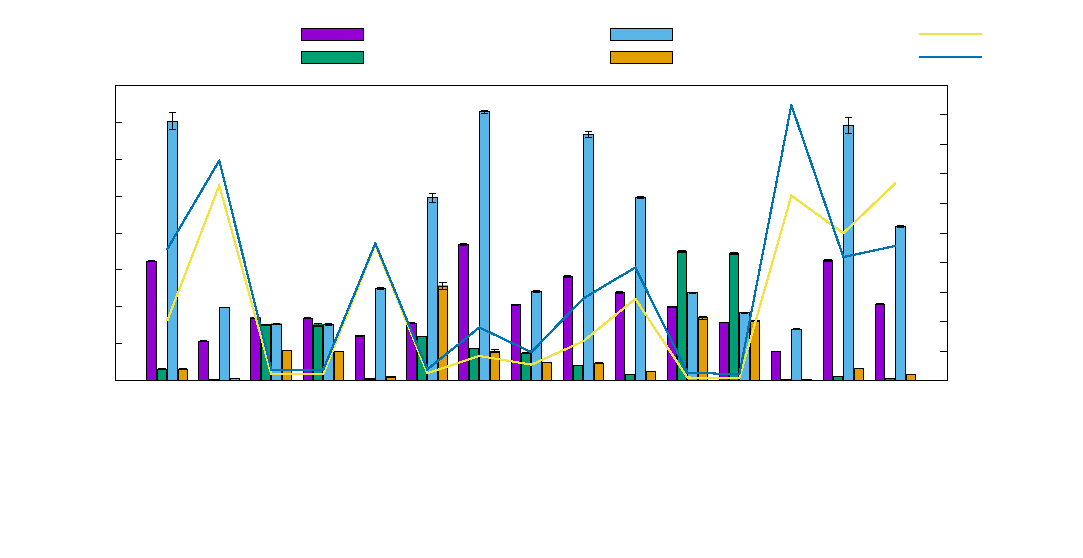
\includegraphics[width={504.00bp},height={252.00bp}]{all-hist-OnlineSetupTimesec}}%
    \gplfronttext
  \end{picture}%
\endgroup

\caption{Circuit Evaluation Time (Setup + Online) of Benchmarks}
\label{fig:graph_all_online_setup}
\end{figure*}

\begin{figure*}[htbp]
\centering
% GNUPLOT: LaTeX picture with Postscript
\begingroup
  \makeatletter
  \providecommand\color[2][]{%
    \GenericError{(gnuplot) \space\space\space\@spaces}{%
      Package color not loaded in conjunction with
      terminal option `colourtext'%
    }{See the gnuplot documentation for explanation.%
    }{Either use 'blacktext' in gnuplot or load the package
      color.sty in LaTeX.}%
    \renewcommand\color[2][]{}%
  }%
  \providecommand\includegraphics[2][]{%
    \GenericError{(gnuplot) \space\space\space\@spaces}{%
      Package graphicx or graphics not loaded%
    }{See the gnuplot documentation for explanation.%
    }{The gnuplot epslatex terminal needs graphicx.sty or graphics.sty.}%
    \renewcommand\includegraphics[2][]{}%
  }%
  \providecommand\rotatebox[2]{#2}%
  \@ifundefined{ifGPcolor}{%
    \newif\ifGPcolor
    \GPcolortrue
  }{}%
  \@ifundefined{ifGPblacktext}{%
    \newif\ifGPblacktext
    \GPblacktextfalse
  }{}%
  % define a \g@addto@macro without @ in the name:
  \let\gplgaddtomacro\g@addto@macro
  % define empty templates for all commands taking text:
  \gdef\gplbacktext{}%
  \gdef\gplfronttext{}%
  \makeatother
  \ifGPblacktext
    % no textcolor at all
    \def\colorrgb#1{}%
    \def\colorgray#1{}%
  \else
    % gray or color?
    \ifGPcolor
      \def\colorrgb#1{\color[rgb]{#1}}%
      \def\colorgray#1{\color[gray]{#1}}%
      \expandafter\def\csname LTw\endcsname{\color{white}}%
      \expandafter\def\csname LTb\endcsname{\color{black}}%
      \expandafter\def\csname LTa\endcsname{\color{black}}%
      \expandafter\def\csname LT0\endcsname{\color[rgb]{1,0,0}}%
      \expandafter\def\csname LT1\endcsname{\color[rgb]{0,1,0}}%
      \expandafter\def\csname LT2\endcsname{\color[rgb]{0,0,1}}%
      \expandafter\def\csname LT3\endcsname{\color[rgb]{1,0,1}}%
      \expandafter\def\csname LT4\endcsname{\color[rgb]{0,1,1}}%
      \expandafter\def\csname LT5\endcsname{\color[rgb]{1,1,0}}%
      \expandafter\def\csname LT6\endcsname{\color[rgb]{0,0,0}}%
      \expandafter\def\csname LT7\endcsname{\color[rgb]{1,0.3,0}}%
      \expandafter\def\csname LT8\endcsname{\color[rgb]{0.5,0.5,0.5}}%
    \else
      % gray
      \def\colorrgb#1{\color{black}}%
      \def\colorgray#1{\color[gray]{#1}}%
      \expandafter\def\csname LTw\endcsname{\color{white}}%
      \expandafter\def\csname LTb\endcsname{\color{black}}%
      \expandafter\def\csname LTa\endcsname{\color{black}}%
      \expandafter\def\csname LT0\endcsname{\color{black}}%
      \expandafter\def\csname LT1\endcsname{\color{black}}%
      \expandafter\def\csname LT2\endcsname{\color{black}}%
      \expandafter\def\csname LT3\endcsname{\color{black}}%
      \expandafter\def\csname LT4\endcsname{\color{black}}%
      \expandafter\def\csname LT5\endcsname{\color{black}}%
      \expandafter\def\csname LT6\endcsname{\color{black}}%
      \expandafter\def\csname LT7\endcsname{\color{black}}%
      \expandafter\def\csname LT8\endcsname{\color{black}}%
    \fi
  \fi
    \setlength{\unitlength}{0.0500bp}%
    \ifx\gptboxheight\undefined%
      \newlength{\gptboxheight}%
      \newlength{\gptboxwidth}%
      \newsavebox{\gptboxtext}%
    \fi%
    \setlength{\fboxrule}{0.5pt}%
    \setlength{\fboxsep}{1pt}%
    \definecolor{tbcol}{rgb}{1,1,1}%
\begin{picture}(10080.00,5040.00)%
    \gplgaddtomacro\gplbacktext{%
      \csname LTb\endcsname%%
      \put(814,1540){\makebox(0,0)[r]{\strut{}$0$}}%
      \put(814,1855){\makebox(0,0)[r]{\strut{}$50$}}%
      \put(814,2171){\makebox(0,0)[r]{\strut{}$100$}}%
      \put(814,2486){\makebox(0,0)[r]{\strut{}$150$}}%
      \put(814,2802){\makebox(0,0)[r]{\strut{}$200$}}%
      \put(814,3117){\makebox(0,0)[r]{\strut{}$250$}}%
      \put(814,3433){\makebox(0,0)[r]{\strut{}$300$}}%
      \put(814,3748){\makebox(0,0)[r]{\strut{}$350$}}%
      \put(814,4064){\makebox(0,0)[r]{\strut{}$400$}}%
      \put(814,4379){\makebox(0,0)[r]{\strut{}$450$}}%
      \put(1416,1408){\rotatebox{-45}{\makebox(0,0)[l]{\strut{}Biometric Matching}}}%
      \put(1886,1408){\rotatebox{-45}{\makebox(0,0)[l]{\strut{}Biometric Matching (Fast)}}}%
      \put(2356,1408){\rotatebox{-45}{\makebox(0,0)[l]{\strut{}Convex Hull}}}%
      \put(2826,1408){\rotatebox{-45}{\makebox(0,0)[l]{\strut{}Count 102}}}%
      \put(3296,1408){\rotatebox{-45}{\makebox(0,0)[l]{\strut{}Count 10s}}}%
      \put(3766,1408){\rotatebox{-45}{\makebox(0,0)[l]{\strut{}Cryptonets (Max Pooling)}}}%
      \put(4236,1408){\rotatebox{-45}{\makebox(0,0)[l]{\strut{}Database Join}}}%
      \put(4706,1408){\rotatebox{-45}{\makebox(0,0)[l]{\strut{}Database Variance}}}%
      \put(5175,1408){\rotatebox{-45}{\makebox(0,0)[l]{\strut{}Histogram}}}%
      \put(5645,1408){\rotatebox{-45}{\makebox(0,0)[l]{\strut{}Inner Product}}}%
      \put(6115,1408){\rotatebox{-45}{\makebox(0,0)[l]{\strut{}k-means}}}%
      \put(6585,1408){\rotatebox{-45}{\makebox(0,0)[l]{\strut{}Longest 102}}}%
      \put(7055,1408){\rotatebox{-45}{\makebox(0,0)[l]{\strut{}Max. Dist. b/w Symbols}}}%
      \put(7525,1408){\rotatebox{-45}{\makebox(0,0)[l]{\strut{}Minimal Points}}}%
      \put(7995,1408){\rotatebox{-45}{\makebox(0,0)[l]{\strut{}MNIST ReLU}}}%
      \put(8465,1408){\rotatebox{-45}{\makebox(0,0)[l]{\strut{}Private Set Intersection}}}%
      \put(9067,1540){\makebox(0,0)[l]{\strut{}$0$}}%
      \put(9067,1946){\makebox(0,0)[l]{\strut{}$2$}}%
      \put(9067,2351){\makebox(0,0)[l]{\strut{}$4$}}%
      \put(9067,2757){\makebox(0,0)[l]{\strut{}$6$}}%
      \put(9067,3162){\makebox(0,0)[l]{\strut{}$8$}}%
      \put(9067,3568){\makebox(0,0)[l]{\strut{}$10$}}%
      \put(9067,3973){\makebox(0,0)[l]{\strut{}$12$}}%
      \put(9067,4379){\makebox(0,0)[l]{\strut{}$14$}}%
    }%
    \gplgaddtomacro\gplfronttext{%
      \csname LTb\endcsname%%
      \put(209,2959){\rotatebox{-270}{\makebox(0,0){\strut{}Communication (MiB)}}}%
      \put(9573,2959){\rotatebox{-270}{\makebox(0,0){\strut{}Improvement (number of times)}}}%
      \csname LTb\endcsname%%
      \put(2602,4867){\makebox(0,0)[r]{\strut{}GMW}}%
      \csname LTb\endcsname%%
      \put(2602,4647){\makebox(0,0)[r]{\strut{}GMW (Vectorized)}}%
      \csname LTb\endcsname%%
      \put(5569,4867){\makebox(0,0)[r]{\strut{}BMR}}%
      \csname LTb\endcsname%%
      \put(5569,4647){\makebox(0,0)[r]{\strut{}BMR (Vectorized)}}%
      \csname LTb\endcsname%%
      \put(8536,4867){\makebox(0,0)[r]{\strut{}GMW Improvement}}%
      \csname LTb\endcsname%%
      \put(8536,4647){\makebox(0,0)[r]{\strut{}BMR Improvement}}%
    }%
    \gplbacktext
    \put(0,0){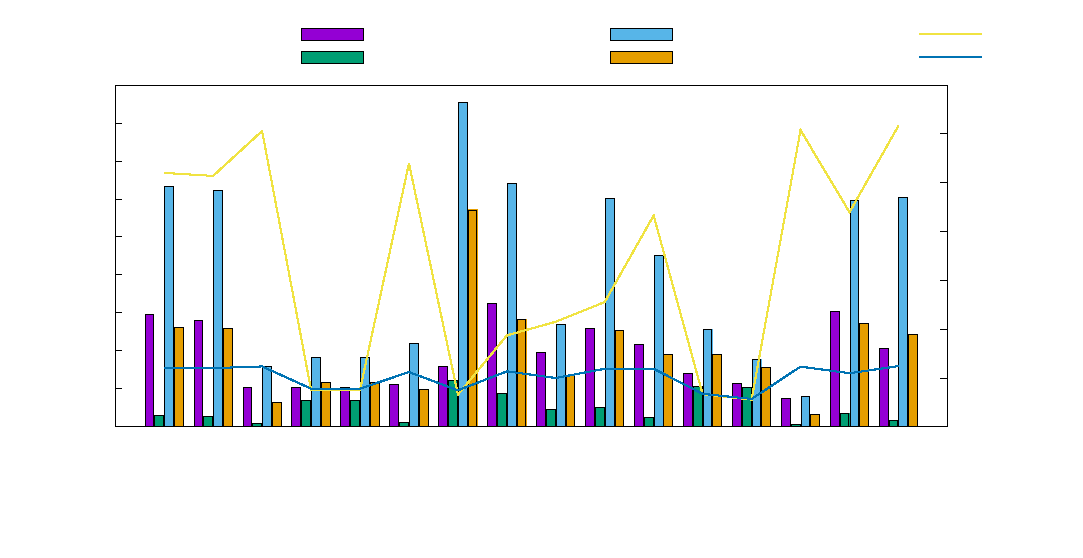
\includegraphics[width={504.00bp},height={252.00bp}]{all-hist-CommunicationMiB}}%
    \gplfronttext
  \end{picture}%
\endgroup

\caption{Communication Size of Benchmarks}
\label{fig:graph_comm_size_time}
\end{figure*}


\begin{figure*}[htbp]
\centering
% GNUPLOT: LaTeX picture with Postscript
\begingroup
  \makeatletter
  \providecommand\color[2][]{%
    \GenericError{(gnuplot) \space\space\space\@spaces}{%
      Package color not loaded in conjunction with
      terminal option `colourtext'%
    }{See the gnuplot documentation for explanation.%
    }{Either use 'blacktext' in gnuplot or load the package
      color.sty in LaTeX.}%
    \renewcommand\color[2][]{}%
  }%
  \providecommand\includegraphics[2][]{%
    \GenericError{(gnuplot) \space\space\space\@spaces}{%
      Package graphicx or graphics not loaded%
    }{See the gnuplot documentation for explanation.%
    }{The gnuplot epslatex terminal needs graphicx.sty or graphics.sty.}%
    \renewcommand\includegraphics[2][]{}%
  }%
  \providecommand\rotatebox[2]{#2}%
  \@ifundefined{ifGPcolor}{%
    \newif\ifGPcolor
    \GPcolortrue
  }{}%
  \@ifundefined{ifGPblacktext}{%
    \newif\ifGPblacktext
    \GPblacktextfalse
  }{}%
  % define a \g@addto@macro without @ in the name:
  \let\gplgaddtomacro\g@addto@macro
  % define empty templates for all commands taking text:
  \gdef\gplbacktext{}%
  \gdef\gplfronttext{}%
  \makeatother
  \ifGPblacktext
    % no textcolor at all
    \def\colorrgb#1{}%
    \def\colorgray#1{}%
  \else
    % gray or color?
    \ifGPcolor
      \def\colorrgb#1{\color[rgb]{#1}}%
      \def\colorgray#1{\color[gray]{#1}}%
      \expandafter\def\csname LTw\endcsname{\color{white}}%
      \expandafter\def\csname LTb\endcsname{\color{black}}%
      \expandafter\def\csname LTa\endcsname{\color{black}}%
      \expandafter\def\csname LT0\endcsname{\color[rgb]{1,0,0}}%
      \expandafter\def\csname LT1\endcsname{\color[rgb]{0,1,0}}%
      \expandafter\def\csname LT2\endcsname{\color[rgb]{0,0,1}}%
      \expandafter\def\csname LT3\endcsname{\color[rgb]{1,0,1}}%
      \expandafter\def\csname LT4\endcsname{\color[rgb]{0,1,1}}%
      \expandafter\def\csname LT5\endcsname{\color[rgb]{1,1,0}}%
      \expandafter\def\csname LT6\endcsname{\color[rgb]{0,0,0}}%
      \expandafter\def\csname LT7\endcsname{\color[rgb]{1,0.3,0}}%
      \expandafter\def\csname LT8\endcsname{\color[rgb]{0.5,0.5,0.5}}%
    \else
      % gray
      \def\colorrgb#1{\color{black}}%
      \def\colorgray#1{\color[gray]{#1}}%
      \expandafter\def\csname LTw\endcsname{\color{white}}%
      \expandafter\def\csname LTb\endcsname{\color{black}}%
      \expandafter\def\csname LTa\endcsname{\color{black}}%
      \expandafter\def\csname LT0\endcsname{\color{black}}%
      \expandafter\def\csname LT1\endcsname{\color{black}}%
      \expandafter\def\csname LT2\endcsname{\color{black}}%
      \expandafter\def\csname LT3\endcsname{\color{black}}%
      \expandafter\def\csname LT4\endcsname{\color{black}}%
      \expandafter\def\csname LT5\endcsname{\color{black}}%
      \expandafter\def\csname LT6\endcsname{\color{black}}%
      \expandafter\def\csname LT7\endcsname{\color{black}}%
      \expandafter\def\csname LT8\endcsname{\color{black}}%
    \fi
  \fi
    \setlength{\unitlength}{0.0500bp}%
    \ifx\gptboxheight\undefined%
      \newlength{\gptboxheight}%
      \newlength{\gptboxwidth}%
      \newsavebox{\gptboxtext}%
    \fi%
    \setlength{\fboxrule}{0.5pt}%
    \setlength{\fboxsep}{1pt}%
    \definecolor{tbcol}{rgb}{1,1,1}%
\begin{picture}(10080.00,5040.00)%
    \gplgaddtomacro\gplbacktext{%
      \csname LTb\endcsname%%
      \put(814,1540){\makebox(0,0)[r]{\strut{}$0$}}%
      \put(814,1895){\makebox(0,0)[r]{\strut{}$20$}}%
      \put(814,2250){\makebox(0,0)[r]{\strut{}$40$}}%
      \put(814,2605){\makebox(0,0)[r]{\strut{}$60$}}%
      \put(814,2960){\makebox(0,0)[r]{\strut{}$80$}}%
      \put(814,3314){\makebox(0,0)[r]{\strut{}$100$}}%
      \put(814,3669){\makebox(0,0)[r]{\strut{}$120$}}%
      \put(814,4024){\makebox(0,0)[r]{\strut{}$140$}}%
      \put(814,4379){\makebox(0,0)[r]{\strut{}$160$}}%
      \put(1437,1408){\rotatebox{-45}{\makebox(0,0)[l]{\strut{}Biometric Matching}}}%
      \put(1928,1408){\rotatebox{-45}{\makebox(0,0)[l]{\strut{}Convex Hull}}}%
      \put(2419,1408){\rotatebox{-45}{\makebox(0,0)[l]{\strut{}Count 102}}}%
      \put(2910,1408){\rotatebox{-45}{\makebox(0,0)[l]{\strut{}Count 10s}}}%
      \put(3401,1408){\rotatebox{-45}{\makebox(0,0)[l]{\strut{}Cryptonets (Max Pooling)}}}%
      \put(3892,1408){\rotatebox{-45}{\makebox(0,0)[l]{\strut{}Database Join}}}%
      \put(4383,1408){\rotatebox{-45}{\makebox(0,0)[l]{\strut{}Database Variance}}}%
      \put(4875,1408){\rotatebox{-45}{\makebox(0,0)[l]{\strut{}Histogram}}}%
      \put(5366,1408){\rotatebox{-45}{\makebox(0,0)[l]{\strut{}Inner Product}}}%
      \put(5857,1408){\rotatebox{-45}{\makebox(0,0)[l]{\strut{}k-means}}}%
      \put(6348,1408){\rotatebox{-45}{\makebox(0,0)[l]{\strut{}Longest 102}}}%
      \put(6839,1408){\rotatebox{-45}{\makebox(0,0)[l]{\strut{}Max. Dist. b/w Symbols}}}%
      \put(7330,1408){\rotatebox{-45}{\makebox(0,0)[l]{\strut{}Minimal Points}}}%
      \put(7821,1408){\rotatebox{-45}{\makebox(0,0)[l]{\strut{}MNIST ReLU}}}%
      \put(8312,1408){\rotatebox{-45}{\makebox(0,0)[l]{\strut{}Private Set Intersection}}}%
      \put(8935,1540){\makebox(0,0)[l]{\strut{}$0$}}%
      \put(8935,1824){\makebox(0,0)[l]{\strut{}$20$}}%
      \put(8935,2108){\makebox(0,0)[l]{\strut{}$40$}}%
      \put(8935,2392){\makebox(0,0)[l]{\strut{}$60$}}%
      \put(8935,2676){\makebox(0,0)[l]{\strut{}$80$}}%
      \put(8935,2960){\makebox(0,0)[l]{\strut{}$100$}}%
      \put(8935,3243){\makebox(0,0)[l]{\strut{}$120$}}%
      \put(8935,3527){\makebox(0,0)[l]{\strut{}$140$}}%
      \put(8935,3811){\makebox(0,0)[l]{\strut{}$160$}}%
      \put(8935,4095){\makebox(0,0)[l]{\strut{}$180$}}%
      \put(8935,4379){\makebox(0,0)[l]{\strut{}$200$}}%
    }%
    \gplgaddtomacro\gplfronttext{%
      \csname LTb\endcsname%%
      \put(209,2959){\rotatebox{-270}{\makebox(0,0){\strut{}Circuit Generation Time (sec)}}}%
      \put(9573,2959){\rotatebox{-270}{\makebox(0,0){\strut{}Improvement (number of times)}}}%
      \csname LTb\endcsname%%
      \put(2536,4867){\makebox(0,0)[r]{\strut{}GMW}}%
      \csname LTb\endcsname%%
      \put(2536,4647){\makebox(0,0)[r]{\strut{}GMW (Vectorized)}}%
      \csname LTb\endcsname%%
      \put(5503,4867){\makebox(0,0)[r]{\strut{}BMR}}%
      \csname LTb\endcsname%%
      \put(5503,4647){\makebox(0,0)[r]{\strut{}BMR (Vectorized)}}%
      \csname LTb\endcsname%%
      \put(8470,4867){\makebox(0,0)[r]{\strut{}GMW Improvement}}%
      \csname LTb\endcsname%%
      \put(8470,4647){\makebox(0,0)[r]{\strut{}BMR Improvement}}%
    }%
    \gplbacktext
    \put(0,0){\includegraphics[width={504.00bp},height={252.00bp}]{all-hist-CircuitGenerationTimesec}}%
    \gplfronttext
  \end{picture}%
\endgroup

\caption{Circuit Generation Time of Benchmarks}
\label{fig:graph_circ_gen_time}
\end{figure*}

\begin{figure*}[htbp]
\centering
% GNUPLOT: LaTeX picture with Postscript
\begingroup
  \makeatletter
  \providecommand\color[2][]{%
    \GenericError{(gnuplot) \space\space\space\@spaces}{%
      Package color not loaded in conjunction with
      terminal option `colourtext'%
    }{See the gnuplot documentation for explanation.%
    }{Either use 'blacktext' in gnuplot or load the package
      color.sty in LaTeX.}%
    \renewcommand\color[2][]{}%
  }%
  \providecommand\includegraphics[2][]{%
    \GenericError{(gnuplot) \space\space\space\@spaces}{%
      Package graphicx or graphics not loaded%
    }{See the gnuplot documentation for explanation.%
    }{The gnuplot epslatex terminal needs graphicx.sty or graphics.sty.}%
    \renewcommand\includegraphics[2][]{}%
  }%
  \providecommand\rotatebox[2]{#2}%
  \@ifundefined{ifGPcolor}{%
    \newif\ifGPcolor
    \GPcolortrue
  }{}%
  \@ifundefined{ifGPblacktext}{%
    \newif\ifGPblacktext
    \GPblacktextfalse
  }{}%
  % define a \g@addto@macro without @ in the name:
  \let\gplgaddtomacro\g@addto@macro
  % define empty templates for all commands taking text:
  \gdef\gplbacktext{}%
  \gdef\gplfronttext{}%
  \makeatother
  \ifGPblacktext
    % no textcolor at all
    \def\colorrgb#1{}%
    \def\colorgray#1{}%
  \else
    % gray or color?
    \ifGPcolor
      \def\colorrgb#1{\color[rgb]{#1}}%
      \def\colorgray#1{\color[gray]{#1}}%
      \expandafter\def\csname LTw\endcsname{\color{white}}%
      \expandafter\def\csname LTb\endcsname{\color{black}}%
      \expandafter\def\csname LTa\endcsname{\color{black}}%
      \expandafter\def\csname LT0\endcsname{\color[rgb]{1,0,0}}%
      \expandafter\def\csname LT1\endcsname{\color[rgb]{0,1,0}}%
      \expandafter\def\csname LT2\endcsname{\color[rgb]{0,0,1}}%
      \expandafter\def\csname LT3\endcsname{\color[rgb]{1,0,1}}%
      \expandafter\def\csname LT4\endcsname{\color[rgb]{0,1,1}}%
      \expandafter\def\csname LT5\endcsname{\color[rgb]{1,1,0}}%
      \expandafter\def\csname LT6\endcsname{\color[rgb]{0,0,0}}%
      \expandafter\def\csname LT7\endcsname{\color[rgb]{1,0.3,0}}%
      \expandafter\def\csname LT8\endcsname{\color[rgb]{0.5,0.5,0.5}}%
    \else
      % gray
      \def\colorrgb#1{\color{black}}%
      \def\colorgray#1{\color[gray]{#1}}%
      \expandafter\def\csname LTw\endcsname{\color{white}}%
      \expandafter\def\csname LTb\endcsname{\color{black}}%
      \expandafter\def\csname LTa\endcsname{\color{black}}%
      \expandafter\def\csname LT0\endcsname{\color{black}}%
      \expandafter\def\csname LT1\endcsname{\color{black}}%
      \expandafter\def\csname LT2\endcsname{\color{black}}%
      \expandafter\def\csname LT3\endcsname{\color{black}}%
      \expandafter\def\csname LT4\endcsname{\color{black}}%
      \expandafter\def\csname LT5\endcsname{\color{black}}%
      \expandafter\def\csname LT6\endcsname{\color{black}}%
      \expandafter\def\csname LT7\endcsname{\color{black}}%
      \expandafter\def\csname LT8\endcsname{\color{black}}%
    \fi
  \fi
    \setlength{\unitlength}{0.0500bp}%
    \ifx\gptboxheight\undefined%
      \newlength{\gptboxheight}%
      \newlength{\gptboxwidth}%
      \newsavebox{\gptboxtext}%
    \fi%
    \setlength{\fboxrule}{0.5pt}%
    \setlength{\fboxsep}{1pt}%
    \definecolor{tbcol}{rgb}{1,1,1}%
\begin{picture}(10080.00,5040.00)%
    \gplgaddtomacro\gplbacktext{%
      \csname LTb\endcsname%%
      \put(1342,1540){\makebox(0,0)[r]{\strut{}$0$}}%
      \put(1342,2108){\makebox(0,0)[r]{\strut{}$500000$}}%
      \put(1342,2676){\makebox(0,0)[r]{\strut{}$1\times10^{6}$}}%
      \put(1342,3243){\makebox(0,0)[r]{\strut{}$1.5\times10^{6}$}}%
      \put(1342,3811){\makebox(0,0)[r]{\strut{}$2\times10^{6}$}}%
      \put(1342,4379){\makebox(0,0)[r]{\strut{}$2.5\times10^{6}$}}%
      \put(1905,1408){\rotatebox{-45}{\makebox(0,0)[l]{\strut{}Biometric Matching}}}%
      \put(2336,1408){\rotatebox{-45}{\makebox(0,0)[l]{\strut{}Biometric Matching (Fast)}}}%
      \put(2767,1408){\rotatebox{-45}{\makebox(0,0)[l]{\strut{}Convex Hull}}}%
      \put(3198,1408){\rotatebox{-45}{\makebox(0,0)[l]{\strut{}Count 102}}}%
      \put(3630,1408){\rotatebox{-45}{\makebox(0,0)[l]{\strut{}Count 10s}}}%
      \put(4061,1408){\rotatebox{-45}{\makebox(0,0)[l]{\strut{}Cryptonets (Max Pooling)}}}%
      \put(4492,1408){\rotatebox{-45}{\makebox(0,0)[l]{\strut{}Database Join}}}%
      \put(4923,1408){\rotatebox{-45}{\makebox(0,0)[l]{\strut{}Database Variance}}}%
      \put(5354,1408){\rotatebox{-45}{\makebox(0,0)[l]{\strut{}Histogram}}}%
      \put(5785,1408){\rotatebox{-45}{\makebox(0,0)[l]{\strut{}Inner Product}}}%
      \put(6216,1408){\rotatebox{-45}{\makebox(0,0)[l]{\strut{}k-means}}}%
      \put(6647,1408){\rotatebox{-45}{\makebox(0,0)[l]{\strut{}Longest 102}}}%
      \put(7079,1408){\rotatebox{-45}{\makebox(0,0)[l]{\strut{}Max. Dist. b/w Symbols}}}%
      \put(7510,1408){\rotatebox{-45}{\makebox(0,0)[l]{\strut{}Minimal Points}}}%
      \put(7941,1408){\rotatebox{-45}{\makebox(0,0)[l]{\strut{}MNIST ReLU}}}%
      \put(8372,1408){\rotatebox{-45}{\makebox(0,0)[l]{\strut{}Private Set Intersection}}}%
      \put(8935,1540){\makebox(0,0)[l]{\strut{}$0$}}%
      \put(8935,1824){\makebox(0,0)[l]{\strut{}$50$}}%
      \put(8935,2108){\makebox(0,0)[l]{\strut{}$100$}}%
      \put(8935,2392){\makebox(0,0)[l]{\strut{}$150$}}%
      \put(8935,2676){\makebox(0,0)[l]{\strut{}$200$}}%
      \put(8935,2960){\makebox(0,0)[l]{\strut{}$250$}}%
      \put(8935,3243){\makebox(0,0)[l]{\strut{}$300$}}%
      \put(8935,3527){\makebox(0,0)[l]{\strut{}$350$}}%
      \put(8935,3811){\makebox(0,0)[l]{\strut{}$400$}}%
      \put(8935,4095){\makebox(0,0)[l]{\strut{}$450$}}%
      \put(8935,4379){\makebox(0,0)[l]{\strut{}$500$}}%
    }%
    \gplgaddtomacro\gplfronttext{%
      \csname LTb\endcsname%%
      \put(209,2959){\rotatebox{-270}{\makebox(0,0){\strut{}Total Gates}}}%
      \put(9573,2959){\rotatebox{-270}{\makebox(0,0){\strut{}Improvement (number of times)}}}%
      \csname LTb\endcsname%%
      \put(2800,4867){\makebox(0,0)[r]{\strut{}GMW}}%
      \csname LTb\endcsname%%
      \put(2800,4647){\makebox(0,0)[r]{\strut{}GMW (Vectorized)}}%
      \csname LTb\endcsname%%
      \put(5767,4867){\makebox(0,0)[r]{\strut{}BMR}}%
      \csname LTb\endcsname%%
      \put(5767,4647){\makebox(0,0)[r]{\strut{}BMR (Vectorized)}}%
      \csname LTb\endcsname%%
      \put(8734,4867){\makebox(0,0)[r]{\strut{}GMW Improvement}}%
      \csname LTb\endcsname%%
      \put(8734,4647){\makebox(0,0)[r]{\strut{}BMR Improvement}}%
    }%
    \gplbacktext
    \put(0,0){\includegraphics[width={504.00bp},height={252.00bp}]{all-hist-TotalGates}}%
    \gplfronttext
  \end{picture}%
\endgroup

\caption{Number of Gates of Benchmarks}
\label{fig:graph_total_gates}
\end{figure*}

\begin{figure*}[htbp]
\centering
\include{graphs/all-hist-OnlineTimesec}
\caption{Online Time of Benchmarks}
\label{fig:graph_online_time}
\end{figure*}

\begin{figure*}[htbp]
\centering
% GNUPLOT: LaTeX picture with Postscript
\begingroup
  \makeatletter
  \providecommand\color[2][]{%
    \GenericError{(gnuplot) \space\space\space\@spaces}{%
      Package color not loaded in conjunction with
      terminal option `colourtext'%
    }{See the gnuplot documentation for explanation.%
    }{Either use 'blacktext' in gnuplot or load the package
      color.sty in LaTeX.}%
    \renewcommand\color[2][]{}%
  }%
  \providecommand\includegraphics[2][]{%
    \GenericError{(gnuplot) \space\space\space\@spaces}{%
      Package graphicx or graphics not loaded%
    }{See the gnuplot documentation for explanation.%
    }{The gnuplot epslatex terminal needs graphicx.sty or graphics.sty.}%
    \renewcommand\includegraphics[2][]{}%
  }%
  \providecommand\rotatebox[2]{#2}%
  \@ifundefined{ifGPcolor}{%
    \newif\ifGPcolor
    \GPcolortrue
  }{}%
  \@ifundefined{ifGPblacktext}{%
    \newif\ifGPblacktext
    \GPblacktextfalse
  }{}%
  % define a \g@addto@macro without @ in the name:
  \let\gplgaddtomacro\g@addto@macro
  % define empty templates for all commands taking text:
  \gdef\gplbacktext{}%
  \gdef\gplfronttext{}%
  \makeatother
  \ifGPblacktext
    % no textcolor at all
    \def\colorrgb#1{}%
    \def\colorgray#1{}%
  \else
    % gray or color?
    \ifGPcolor
      \def\colorrgb#1{\color[rgb]{#1}}%
      \def\colorgray#1{\color[gray]{#1}}%
      \expandafter\def\csname LTw\endcsname{\color{white}}%
      \expandafter\def\csname LTb\endcsname{\color{black}}%
      \expandafter\def\csname LTa\endcsname{\color{black}}%
      \expandafter\def\csname LT0\endcsname{\color[rgb]{1,0,0}}%
      \expandafter\def\csname LT1\endcsname{\color[rgb]{0,1,0}}%
      \expandafter\def\csname LT2\endcsname{\color[rgb]{0,0,1}}%
      \expandafter\def\csname LT3\endcsname{\color[rgb]{1,0,1}}%
      \expandafter\def\csname LT4\endcsname{\color[rgb]{0,1,1}}%
      \expandafter\def\csname LT5\endcsname{\color[rgb]{1,1,0}}%
      \expandafter\def\csname LT6\endcsname{\color[rgb]{0,0,0}}%
      \expandafter\def\csname LT7\endcsname{\color[rgb]{1,0.3,0}}%
      \expandafter\def\csname LT8\endcsname{\color[rgb]{0.5,0.5,0.5}}%
    \else
      % gray
      \def\colorrgb#1{\color{black}}%
      \def\colorgray#1{\color[gray]{#1}}%
      \expandafter\def\csname LTw\endcsname{\color{white}}%
      \expandafter\def\csname LTb\endcsname{\color{black}}%
      \expandafter\def\csname LTa\endcsname{\color{black}}%
      \expandafter\def\csname LT0\endcsname{\color{black}}%
      \expandafter\def\csname LT1\endcsname{\color{black}}%
      \expandafter\def\csname LT2\endcsname{\color{black}}%
      \expandafter\def\csname LT3\endcsname{\color{black}}%
      \expandafter\def\csname LT4\endcsname{\color{black}}%
      \expandafter\def\csname LT5\endcsname{\color{black}}%
      \expandafter\def\csname LT6\endcsname{\color{black}}%
      \expandafter\def\csname LT7\endcsname{\color{black}}%
      \expandafter\def\csname LT8\endcsname{\color{black}}%
    \fi
  \fi
    \setlength{\unitlength}{0.0500bp}%
    \ifx\gptboxheight\undefined%
      \newlength{\gptboxheight}%
      \newlength{\gptboxwidth}%
      \newsavebox{\gptboxtext}%
    \fi%
    \setlength{\fboxrule}{0.5pt}%
    \setlength{\fboxsep}{1pt}%
    \definecolor{tbcol}{rgb}{1,1,1}%
\begin{picture}(10080.00,5040.00)%
    \gplgaddtomacro\gplbacktext{%
      \csname LTb\endcsname%%
      \put(814,1540){\makebox(0,0)[r]{\strut{}$0$}}%
      \put(814,2013){\makebox(0,0)[r]{\strut{}$50$}}%
      \put(814,2486){\makebox(0,0)[r]{\strut{}$100$}}%
      \put(814,2960){\makebox(0,0)[r]{\strut{}$150$}}%
      \put(814,3433){\makebox(0,0)[r]{\strut{}$200$}}%
      \put(814,3906){\makebox(0,0)[r]{\strut{}$250$}}%
      \put(814,4379){\makebox(0,0)[r]{\strut{}$300$}}%
      \put(1445,1408){\rotatebox{-45}{\makebox(0,0)[l]{\strut{}Biometric Matching}}}%
      \put(1945,1408){\rotatebox{-45}{\makebox(0,0)[l]{\strut{}Convex Hull}}}%
      \put(2444,1408){\rotatebox{-45}{\makebox(0,0)[l]{\strut{}Count 102}}}%
      \put(2943,1408){\rotatebox{-45}{\makebox(0,0)[l]{\strut{}Count 10s}}}%
      \put(3443,1408){\rotatebox{-45}{\makebox(0,0)[l]{\strut{}Cryptonets (Max Pooling)}}}%
      \put(3942,1408){\rotatebox{-45}{\makebox(0,0)[l]{\strut{}Database Join}}}%
      \put(4441,1408){\rotatebox{-45}{\makebox(0,0)[l]{\strut{}Database Variance}}}%
      \put(4941,1408){\rotatebox{-45}{\makebox(0,0)[l]{\strut{}Histogram}}}%
      \put(5440,1408){\rotatebox{-45}{\makebox(0,0)[l]{\strut{}Inner Product}}}%
      \put(5939,1408){\rotatebox{-45}{\makebox(0,0)[l]{\strut{}k-means}}}%
      \put(6438,1408){\rotatebox{-45}{\makebox(0,0)[l]{\strut{}Longest 102}}}%
      \put(6938,1408){\rotatebox{-45}{\makebox(0,0)[l]{\strut{}Max. Dist. b/w Symbols}}}%
      \put(7437,1408){\rotatebox{-45}{\makebox(0,0)[l]{\strut{}Minimal Points}}}%
      \put(7936,1408){\rotatebox{-45}{\makebox(0,0)[l]{\strut{}MNIST ReLU}}}%
      \put(8436,1408){\rotatebox{-45}{\makebox(0,0)[l]{\strut{}Private Set Intersection}}}%
      \put(9067,1540){\makebox(0,0)[l]{\strut{}$0$}}%
      \put(9067,1946){\makebox(0,0)[l]{\strut{}$5$}}%
      \put(9067,2351){\makebox(0,0)[l]{\strut{}$10$}}%
      \put(9067,2757){\makebox(0,0)[l]{\strut{}$15$}}%
      \put(9067,3162){\makebox(0,0)[l]{\strut{}$20$}}%
      \put(9067,3568){\makebox(0,0)[l]{\strut{}$25$}}%
      \put(9067,3973){\makebox(0,0)[l]{\strut{}$30$}}%
      \put(9067,4379){\makebox(0,0)[l]{\strut{}$35$}}%
    }%
    \gplgaddtomacro\gplfronttext{%
      \csname LTb\endcsname%%
      \put(209,2959){\rotatebox{-270}{\makebox(0,0){\strut{}Setup Time (sec)}}}%
      \put(9573,2959){\rotatebox{-270}{\makebox(0,0){\strut{}Improvement (number of times)}}}%
      \csname LTb\endcsname%%
      \put(2602,4867){\makebox(0,0)[r]{\strut{}GMW}}%
      \csname LTb\endcsname%%
      \put(2602,4647){\makebox(0,0)[r]{\strut{}GMW (Vectorized)}}%
      \csname LTb\endcsname%%
      \put(5569,4867){\makebox(0,0)[r]{\strut{}BMR}}%
      \csname LTb\endcsname%%
      \put(5569,4647){\makebox(0,0)[r]{\strut{}BMR (Vectorized)}}%
      \csname LTb\endcsname%%
      \put(8536,4867){\makebox(0,0)[r]{\strut{}GMW Improvement}}%
      \csname LTb\endcsname%%
      \put(8536,4647){\makebox(0,0)[r]{\strut{}BMR Improvement}}%
    }%
    \gplbacktext
    \put(0,0){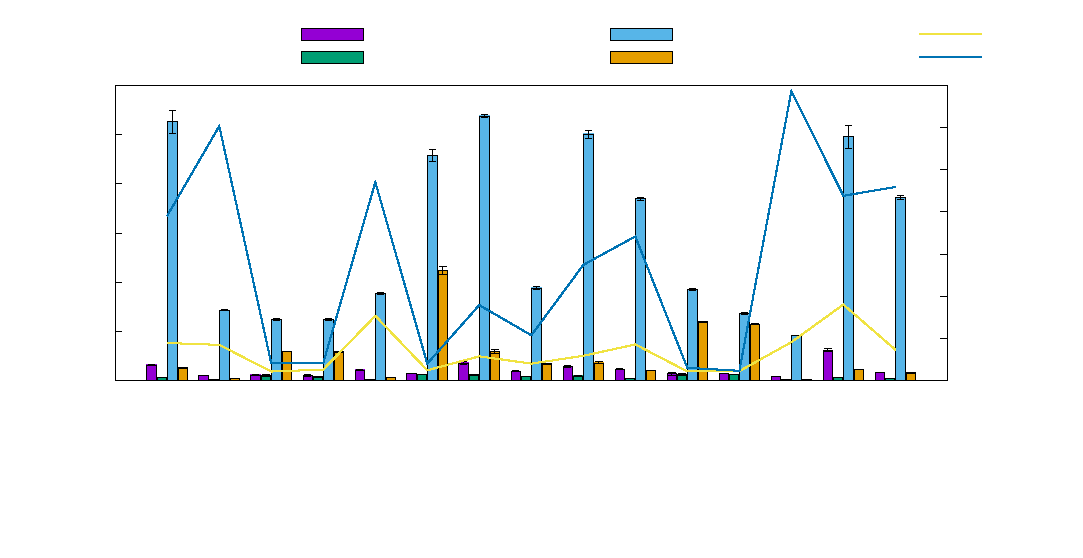
\includegraphics[width={504.00bp},height={252.00bp}]{all-hist-SetupTimesec}}%
    \gplfronttext
  \end{picture}%
\endgroup

\caption{Setup Time of Benchmarks}
\label{fig:graph_setup_time}
\end{figure*}


